% This LaTeX was auto-generated from MATLAB code.
% To make changes, update the MATLAB code and export to LaTeX again.

\documentclass{article}

\usepackage[utf8]{inputenc}
\usepackage[T1]{fontenc}
\usepackage{lmodern}
\usepackage{graphicx}
\usepackage{color}
\usepackage{hyperref}
\usepackage{amsmath}
\usepackage{amsfonts}
\usepackage{epstopdf}
\usepackage[table]{xcolor}
\usepackage{matlab}

\sloppy
\epstopdfsetup{outdir=./}
\graphicspath{ {./submission_images/} }

\matlabmultipletitles

\begin{document}

\matlabtitle{ECE1150 ASSIGNMENT4}

\begin{par}
\begin{flushleft}
Yinhao Qian @ University of Pittsburgh
\end{flushleft}
\end{par}

\begin{matlabcode}
%please ignore this block
answer = @(num,unit) fprintf("<strong> ANSWER: %s [%s]" + ...
    " </strong>\n",mat2str(num),unit);
question = @() eval("clearvars -except answer question");
\end{matlabcode}


\matlabtitle{Q1A}

\begin{matlabcode}
question();
A = 2;%[] amplitude
f = (48*pi)/(2*pi);%[Hz] frequency
phi = 0;%[] phase
samplingRate = 2*f;%[Hz] minimum sampling rate
answer(samplingRate,"Hz");
\end{matlabcode}
\begin{matlaboutput}
 ANSWER: 48 [Hz] 
\end{matlaboutput}

\matlabtitle{Q1B}

\begin{par}
\begin{flushleft}
I assume this question is asking the quantization sequence rather than the quantization levels, as the quantiztion levels are given.
\end{flushleft}
\end{par}

\begin{matlabcode}
H = 2;%[] max cap
L = -2;%[] min cap
N = 8;%[] quatization levels
\end{matlabcode}

\begin{par}
\begin{flushleft}
Size of quantization intervals:
\end{flushleft}
\end{par}

\begin{matlabcode}
S = (H-L)/N;%[] size of quantization intervals
answer(S,"");
\end{matlabcode}
\begin{matlaboutput}
 ANSWER: 0.5 [] 
\end{matlaboutput}

\begin{par}
\begin{flushleft}
Sequence of quantization intervals:
\end{flushleft}
\end{par}

\begin{matlabcode}
sequence = -2+S:S:2-S;
answer(sequence,"")
\end{matlabcode}
\begin{matlaboutput}
 ANSWER: [-1.5 -1 -0.5 0 0.5 1 1.5] [] 
\end{matlaboutput}

\matlabtitle{Q1C}

\begin{matlabcode}
maxError = S/2;%[] maximum quantization error
answer(maxError,"");
\end{matlabcode}
\begin{matlaboutput}
 ANSWER: 0.25 [] 
\end{matlaboutput}

\matlabtitle{Q1D}

\begin{matlabcode}
b = log2(N);%[] bits needed to represent each quantization level
answer(b,"");
\end{matlabcode}
\begin{matlaboutput}
 ANSWER: 3 [] 
\end{matlaboutput}

\matlabtitle{Q1E}

\begin{matlabcode}
sampledValue = 1.1;%[] sampled value
index = find(sequence>sampledValue,1)-1;%[] 0-based index
binaryCode = dec2bin(index);%[] binary code
answer(binaryCode,"")
\end{matlabcode}
\begin{matlaboutput}
 ANSWER: '110' [] 
\end{matlaboutput}

\matlabtitle{Q1F}

\begin{par}
\begin{flushleft}
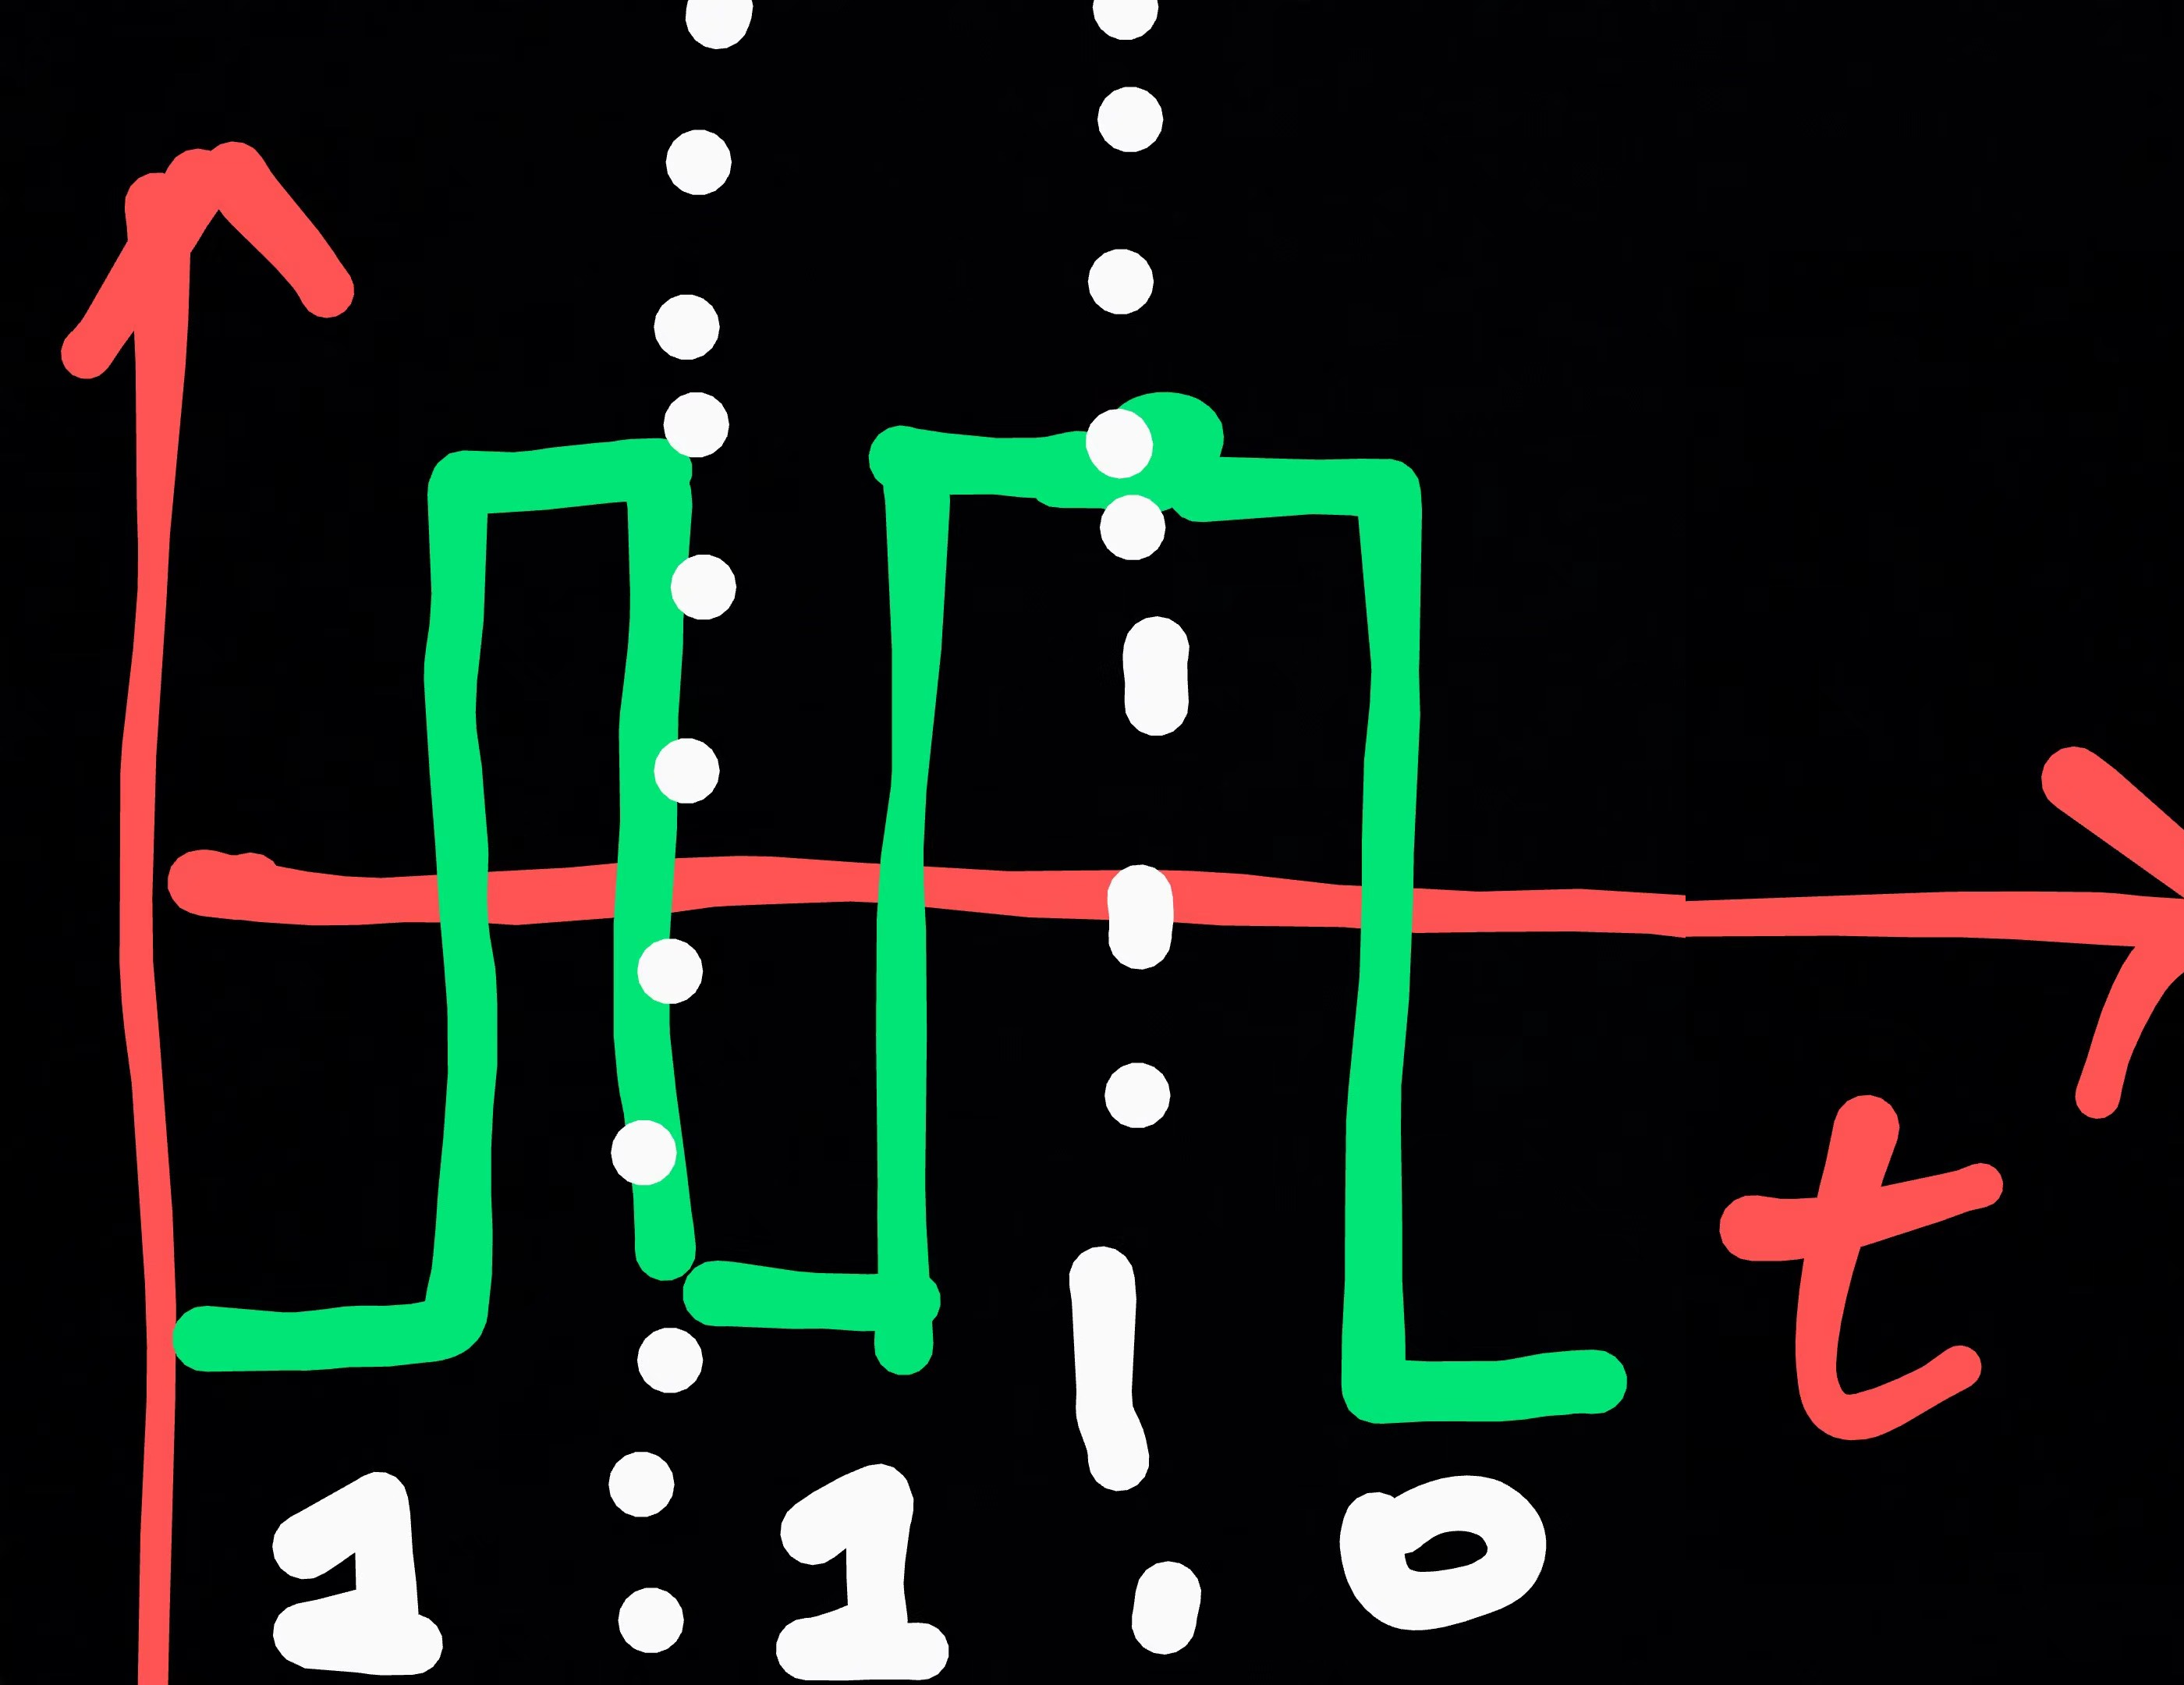
\includegraphics[width=\maxwidth{50.17561465127948em}]{image_0}
\end{flushleft}
\end{par}


\matlabtitle{Q2A}

\begin{par}
\begin{flushleft}
I'm not sure if the topics of QAM and multiplexing is completed covered by the due day of this homework, but I'll try my best to answer this question.
\end{flushleft}
\end{par}

\begin{matlabcode}
question();
maxSymbolRate = 5e9;%[symbols/s]
answer(maxSymbolRate,"symbols/s");
\end{matlabcode}
\begin{matlaboutput}
 ANSWER: 5000000000 [symbols/s] 
\end{matlaboutput}

\matlabtitle{Q2B}

\begin{matlabcode}
k = 2;
baud = maxSymbolRate*k;
answer(baud,"bits/s");
\end{matlabcode}
\begin{matlaboutput}
 ANSWER: 10000000000 [bits/s] 
\end{matlaboutput}

\matlabtitle{Q2C}

\begin{matlabcode}
k = 4;
baud = maxSymbolRate*k;
answer(baud,"bits/s");
\end{matlabcode}
\begin{matlaboutput}
 ANSWER: 20000000000 [bits/s] 
\end{matlaboutput}


\begin{matlabcode}
%please ignore this block
export("submission.mlx","submission.tex");
\end{matlabcode}

\end{document}
